\begin{figure}[h!]
    \centering
    \begin{subfigure}[b]{0.23\textwidth}
        \centering
        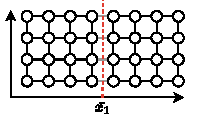
\includegraphics[width=\textwidth]{images/coord_1.drawio.svg.pdf}
        \caption{}
        \label{fig:coord_1}
    \end{subfigure}
    \hfill
    \begin{subfigure}[b]{0.23\textwidth}
        \centering
        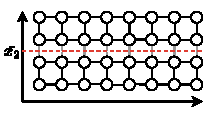
\includegraphics[width=\textwidth]{images/coord_2.drawio.svg.pdf}
        \caption{}
        \label{fig:coord_2}
    \end{subfigure}
    \caption{Bisection of the graph along the $x_1$-axis, resulting in a 4-edge cut (left),
    and along the $x_2$-axis, resulting in 8-edge cut (right). The $x_1$-axis bisection is selected.}
    \label{fig:coord}
\end{figure}